%%%\chapter{INTRODUCTION}

\section{Background and Motivation}
The nature and quality of the service requirements of the Internet have changed drastically in the last two decades. According to the statistics of Cisco's Visual Networking Index Forecast (2015-2020) \cite{winCisco}: high bandwidth traffic makes 70\% of IP traffic today and would rise to 82\% by 2020. Applications such as IPTV (PPStream, PPLive), global transfers of analytical datasets, transport of ultra-high 3D resolution data used in scientific and medical research need high bandwidth, fast and reliable communication. In the first International Workshop on Protocols for high speed and long distance networks \cite{winfirst}, several presentations were put forward on requiring the transfer of multi-GB and multi-TB datasets over the gigabit networks per second. 

Transmission Control Protocol (TCP), which is a most widely used transport protocol, is used in these scenarios; and therefore its import aspect -- Flow and Congestion control mechanism should perform well in high bandwidth networks. But, as bandwidth or the delay goes on increasing, TCP shows low performance and reacts adversely mainly because of its conservative congestion avoidance algorithm. The slow-start phase of TCP increases the transfer speed exponentially and causes a large number of packet drops once the channel capacity is filled. TCP wastes a considerable amount of bandwidth once congestion avoidance phase is reached due to detection of packet loss taking it a long time to fill the capacity (refer figure \ref{tcp}).

\begin{figure}[htbp]
\label{tcp}
\begin{center}
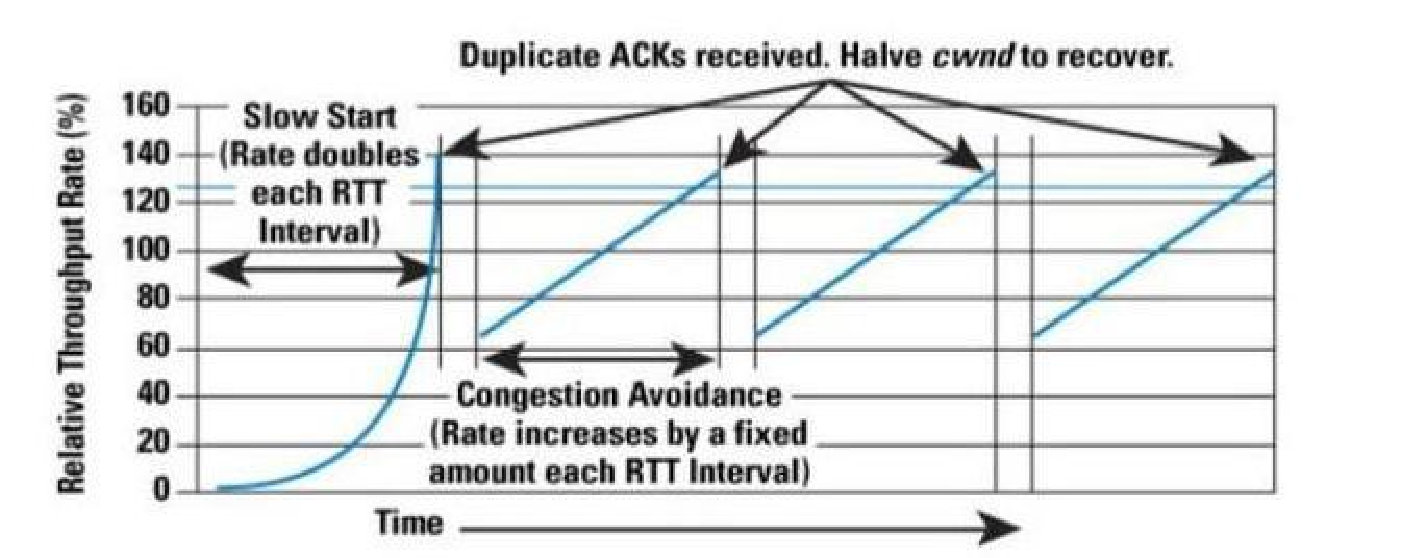
\includegraphics[width=5.5in]{Figures/img11}
\caption{TCP behavior in high bandwidth networks \cite{ipj}}
\end{center}
\end{figure}

To address this performance issue of TCP in high speed networks, researchers have come up with many proposals for modifying the congestion avoidance algorithm in past two to three decades. Some of them are High Speed TCP \cite{floyd2003highspeed}, H-TCP \cite{leith2004h}, BIC TCP \cite{xu2004binary}, CUBIC TCP \cite{ha2008cubic}, YeaH TCP \cite{baiocchi2007yeah}, Compound TCP \cite{tan2006compound}. But none of these variants act as a universal mechanism for improving challenges such as efficiency and bandwidth utilization in ever changing high bandwidth Internet \cite{li2007experimental} \cite{alrshah2014comparative}. 
%The research history also shows that fountain codes increases the reliability and minimizes the effects of packet loss \cite{molnar2009comprehensive} in network communication.

\noindent
\textbf{Motivation:} 
Concerning the limitations of TCP, there is a significant justification on replacing the concept of this protocol, specifically its congestion control mechanism. Some ideas have been proposed by Global Environment for Network Innovations (GENI), suggesting a future Internet without congestion control mechanism, in which they motivate to use efficient erasure coding schemes to recover packet loss or error. Researchers have also implemented the erasure codes in the network communication. Sundararajan et al.,\cite{sundararajan2011network} use TCP/NC that incorporates network coding into TCP with only minor changes in the protocol stack. It helped to increase efficiency by correcting packets that got lost due to congestion, but the congestion avoidance mechanism was not replaced totally. L{\'o}pez et al., \cite{lopez2005game} investigated a fountain code based protocol using game theory. But, its performance in the network was similar to the performance of TCP. Botos et al., \cite{botocs2010analysis} presented new transport protocol for high loss environments using rateless codes making modifications to slow start and congestion avoidance phase. These modifications resulted to avoid the dramatic decrease of sending rate in high packet loss environment. Bonald et al.,\cite{bonald2009law} analyzed the network behavior in the absence of congestion control and their results confuted the common belief that network communication without congestion control would collapse. Thus, omitting congestion control and applying erasure codes show one of a realistic approach to network communication.

This research is motivated by the above observations. We take a practical step in implementing a new transport protocol, by applying fountain codes on the application layer of Internet Protocol(IP) stack, called as Application Layer Forward Error Correction based User Datagram Protocol (ALFEC--UDP). 

We use User Datagram Protocol (UDP) as a transport protocol, since, it increases the speed of data transport by providing least transmission delay and best effort service. UDP reduces delay in transmission by omitting the connection process, flow control, error recovery and retransmission mechanisms. As a secondary benefit, UDP does not care about the congestion avoidance mechanism while transferring data on high bandwidth networks. 

As applications using high bandwidth capacity links require reliability, packet loss recovery and error correction mechanism is implemented by applying erasure codes at the application layer of UDP. Rateless erasure codes unlike traditional erasure codes, do not have fixed coding rate and thus can a produce potentially infinite stream of the codeword as long as it is necessary for the actual transmission to complete. The decoder can recover the sent information from any subset of the encoded stream, which is slightly larger than the original message. When the loss is experienced in the network, receiver hosts would only have to collect a subset of the encoded stream until they obtain a require amount of it to process decoding. 

The first practical rateless codes introduced were Luby Transform (LT) codes. But, they failed to provide low complexity in encoding and decoding operations. We propose the use of Raptor erasure codes, \cite{shokrollahi2006raptor} which has been recently declared to be one of the most powerful rateless erasure codes in Forward Error Correction (FEC) axis, in this research. Being an extension to LT codes, they offer linear time encoding and decoding complexity thus decreasing the processing time.

\section{Contributions:} 
The contributions of this research include:
\begin{itemize}
\item Design of ALFEC--UDP protocol for reliable data transport in high speed networks.
\item Implement the protocol to analyze and demonstrate its efficiency through comparisons with present high speed TCP variants.
\end{itemize}
%Since the use of UDP as transport protocol is increasing rapidly in today's Internet. In terms of flows, the statistical survey of Center for Applied Internet Data Analysis (CAIDA) \cite{caida} observed that there is one TCP flow for every three UDP flows in today's Internet. 

%Despite of all benefits, the mechanism of correcting packet error and packet loss recovery are lacking in UDP. 





\begin{comment}
%In the network communication researchers provide efficient solutions, but fail to act as a universal mechanism considering heterogeneous and ever changing network conditions \cite{lai2010enhancing} \cite{mascolo2001tcp} \cite{li2007experimental} \cite{molnar2009comprehensive}. In a high bandwidth environment TCP suffers from random packet losses because of the time needed for it to get feedback from the receiver. After a packet loss, TCP goes into congestion avoidance state, where the congestion window size is increased by one unit per round-trip time (RTT). This takes a long time to maximize the capacity of the channel. 
%When the threshold is small, increasing the window by a small amount is a reasonable thing to do, but when the window is very large, each acknowledgment adds a small increase in the window size. 
%In cases like packet loss, duplicate acknowledgment though threshold cut into half, requires an extraordinary large number of RTT to utilize the resources fully, making TCP to behave very sluggish. Since the window based mechanism of current TCP implementations is not suitable for achieving high link utilization, researchers have proposed modifications to TCP and UDP to improve the performance that it presents in high bandwidth links.

%In response of TCP congestion control problems in 
%\todo{remove "in the networks with"}
%high bandwidth networks, and lack of error recovery mechanism in UDP, we try to introduce raptor code in the network communication.  It would useful to allocate (possibly, depending on the actual loss rate) a small fraction of the bandwidth to send redundant packets. The sender computes a small number of redundant packets on every group of original data packets, and appends these packets at the end of the group. During this time, if the group is complete and some of the redundant packets are available at the receiver side, then the missing one(s) can be recovered without the need for an explicit retransmission (this would be equivalent to a fast retransmit). The network would be utilized fully and there is no need to address the issues like acknowledgment overhead, retransmission of the missing packets, and packet reordering.

\par
Digital Fountain's raptor FEC is highly advanced and flexible mechanism that ensures the efficient and error-free delivery of both multimedia and data files even though in the presence of wide variety of network impairments. In modern wireless and wired communication system, FEC codes are employed for efficient transmission of data over noisy channels \cite{palanisamy2008performance} \cite{palanisamy2008performance1} \cite{molnar2013data}. FEC are family of erasure correction codes with capability of recovering missing or lost data at the application, transport and physical layer to provide reliability and guarantee of error free delivery in end to end communication. Thus the most advanced FEC codes, raptor, would provide reliability to the UDP transport protocol with error-correction capability and efficient error free delivery of the data.

 The purpose of this study is to evaluate the performance of raptor codes to minimize the effects of these packet losses in UDP. In order to realize this aim, following sub-problems were tackled:



\subsection{Sub-problem 1:}
Raptor codes required testing to ensure its correct working and efficiency, independently. Therefore in this research, the design of raptor codes as stand-alone modules were carried out.
\subsection{Sub-problem 2:}
Once raptor codes had been designed and tested, it was necessary to integrate its error correcting scheme into a functional module in ns-3, necessitating the implementation of raptor codes in ns-3.


%\section{Contributions}
%This research introduces the data transport using fountain codes along with replacement of TCP with an effective FC--UDP at the application layer. This thesis will also analyze the performance of FC--UDP with TCP\textquotesingle s high-speed congestion control variants. The variants used for comparison are TCP--Highspeed, TCP--Westwood, TCP--Hybla.
%\todo[inline]{Contributions should be listed in more details. One of the contributions is an implementation of the Raptor code}

%\section{Research Objectives}
%The objective of this research was to demonstrate the efficiency of raptor code in providing effective data transport together reducing packet loss in UDP. The extension of ns-3, through introduction of raptor code libraries was carried out. The usefulness and relevance of raptor codes to transport data in the network communication were shown.

\section{Delimitations}
\begin{itemize}
\item The research work was limited to the interaction of transport and the application layer.
\item Point to point data transmission was considered.
\item Packet lost and reordered, but not corrupted ones were considered.
\end{itemize}
\end{comment}
\section{Thesis Organization}
 In chapter 2, the related work on the development of UDP as a transport protocol and applications of raptor codes in network communication is presented. Chapter 3 discusses the terminology of fountain codes, erasure channel, and systematic raptor codes. In Chapter 4, we discuss the design and methodology of our proposed protocol. Chapter 5 presents the simulation topology, experiment results, and analysis of our protocol. Chapter 6 concludes and presents the scope for further work.
